\section{Introduction}

Asynchronous audio communication (AAC) is rapidly becoming available to mass audiences through social platforms such as WhatsApp, iMessage, and Facebook. 
While text is still by far the most prevalent (and often most convenient) mode of communication on the Internet, audio is desirable in many situations because of its ability to convey more expression and nuance than text.
For instance, Mayer's work on multimedia learning \cite{mayer} indicates that audio communication is particularly useful for managing cognitive load where material is primarily conveyed visually (e.g., by pointing), and in situations where an emotional connection between speaker and listener is desirable.
AAC therefore holds considerable potential for improving online education, where voice communication has been demonstrated to improve student-student and student-instructor engagement as well as a sense of the instructor's social presence \cite{ice,oomen,tu}. 
Our research is primarily motivated by the implications of AAC as a peer-to-peer educational tool, though it is also applicable to other collaborative settings, such as instructor authoring.

\begin{figure}
	\centering
	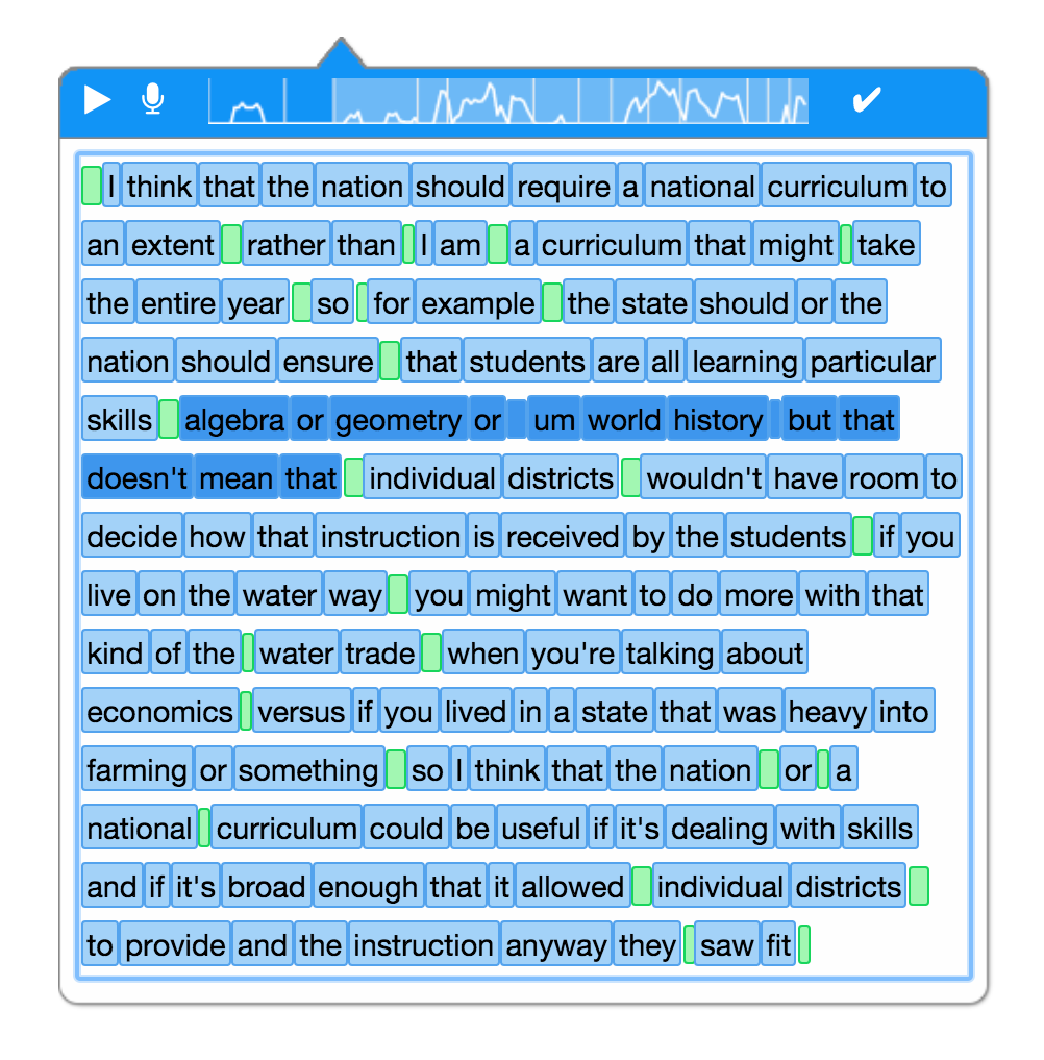
\includegraphics[width=\columnwidth,keepaspectratio]{figures/large_screenshot}
	\caption{The user interface for SimpleSpeech presents an automatically-generated transcription of a voice comment, which can then be manipulated through normal word-processing operations, such as selection, deletion, and insertion. Word and pause tokens are mapped with audio via time alignment data.ß}~\label{fig:overview_shot}
\end{figure}

The problem with replacing textual communication with speech, however, is that speakers may face difficulty articulating their ideas vocally.
For instance, Marriott and Hiscock's study using Wimba voice boards for discussion forums found that students overwhelmingly preferred text over speech comments, in part because it required them to speak fluently without making errors \cite{wimba}.
Since this problem affects students even in physical classrooms, it could certainly prevent some learners from participating in online oral discussions.
AAC platforms in such situations, then, must somehow compensate for the linearity and immutability of audio on the production side.

Our solution is to provide lightweight, easy-to-use editing tools based on automatic speech recognition (ASR)-generated transcripts.
Many prior studies have utilized transcription to assist in audio editing \cite{casares,rubin,whittaker_semantic}, but only recently has fast, live editing become possible through advances in ASR technology \cite{baker,saon}.
We implemented a similar audio production tool, SimpleSpeech, that allows users to delete and insert segments of the recording in real-time, simplifying quick word-level editing even when transcription errors are present.

Qualitative evidence indicates that SimpleSpeech's simplified interface gave users enough control over the editing process and enabled them to produce more polished audio comments, but that these benefits came at the price of elevated mental workload and formality.
Further quantitative investigation on these themes showed that the workload of recording voice messages was significantly less with editing functionality, demonstrating that SimpleSpeech would be a valuable enhancement to online audio communication platforms.
Finally, linguistic characteristics of messages created using AAC are also discussed in comparison to other forms of communication, leading to new considerations and insights on optimal applications of this technology.
